\chapter{Introduction} \label{sec:chapter_intro}
Anomaly detection is an important task in environments where we have a good knowledge of what is the normal behaviour, but we know very little about the behaviour of yet unseen or otherwise abnormal events -- anomalies. The reasons for this can be numerous: either there is no common generating principle behind anomalies and each new anomaly may be very different from those that we have yet seen, or the acquisition of anomalous data is too expensive or downright impossible (an example of this might be an industrial process). Usually, there is a disbalance in the number of labeled normal and anomalous data samples that are available to us, and sometimes no anomalies are available at all. While it might be tempting to solve anomaly detection as supervised binary classification, for the reasons listed above, a supervised classifier is likely to be unrobust to actual anomalies that it will encounter in a production environment. Together with an ever-increasing volume of collected data and available computing power, this motivates the development of specialized methods for automatic anomaly detection. What these methods have in common is that they learn a model of only the normal data, and detect anomalies as deviations from this model. 

The actions taken after an anomaly is detected might be varied. Sometimes, the anomaly might be considered to be an erroneous measurement and as such is ignored, which is the case of some of the earliest scientific essays~\cite{glaisher1873rejection,edgeworth1887xli} on the topic of anomaly detection. In other cases, a preventive measure must be taken in order to mitigate unwanted behaviour, such as the case of cybersecurity~\cite{liao2013intrusion, vanerio2017ensemble,xin2018machine}, fraud detection~\cite{bolton2002statistical, perols2011financial, ahmed2016survey}, medical diagnosis~\cite{tarassenko1995novelty, wong2003bayesian, iakovidis2018detecting,zhou2019anomalynet} or industrial process monitoring~\cite{mahmoudi2019layerwise, bai2020anomaly, choi2020gan}. Finally, detected anomalies might drive forward scientific discovery in astronomy~\cite{protopapas2006finding}, plasma physics~\cite{vskvara2020detection}, chemistry~\cite{oprea2002chemical} or particle physics~\cite{fraser2022challenges}.

There are countless models and algorithms for anomaly detection, tackling the problem from different angles based on the basic principle of the algorithm, the expected nature of the data, and the application domain. There are methods based on random forests\,\cite{liu2008isolation}, the k--nearest neighbors algorithm\,\cite{harmeling2006outliers}, Gaussian mixture models\,\cite{mahadevan2010anomaly}, clustering neural networks\,\cite{schlegl2017unsupervised}, histogram estimation\,\cite{pevny2016loda}, kernel density estimates\,\cite{latecki2007outlier} or support vector machines\,\cite{scholkopf2001estimating}. A comprehensive overview of anomaly detection methods is presented in studies such as\,\cite{pimentel2014review,goldstein2016comparative,lazarevic2003comparative,chandola2009anomaly,campos2016evaluation} where the authors compare several existing methods on benchmark datasets. Our own overview of some classical anomaly detectors follows in Chapter~\ref{sec:chapter_shallow}.


Deep generative models have recently attracted a lot of attention due to their ability to produce (generate) very high-quality artificial images that resemble those from the training dataset. Since the seminal papers\,\cite{goodfellow2014gan,kingma2013vae,dinh2014nice} on the main types of generative models have been published, a myriad of improvements and tweaks have been proposed. While the original purpose of generative models was not aimed towards anomaly detection, some of them were redesigned for it. Most of the comparative studies of anomaly detectors however do not include methods based on (deep) neural networks and especially not generative models. The probably most recent and complete overview of deep generative models can be found at~\cite{ruff2020unifying}.
This text intends to collect some (but definitely not all) of the relevant information on deep generative models in one place and assess the potential suitability of the different generative models to the task of anomaly detection.

\section{What is anomaly detection?} \label{sec:ad_definition}
Anomaly detection has been extensively studied under many different names: outlier detection~\cite{knorr98algorithms,hodge2004survey}, novelty detection~\cite{pimentel2014review}, one-class classification~\cite{ruff2018deep} or out-of-distribution detection~\cite{liang2017enhancing}. There is a small distinction between these terms based on the application domain, but the methods used to solve the problems they present are in principle the same. In the same vein, the terms outlier, novelty, and anomaly may have a slightly different meaning in some publications, but at the same time are often used interchangeably. In this text, we will resort to the use of the last term. An often cited definition of what constitutes an anomaly is ``an observation which deviates so much from other observations as to arouse suspicion that it was generated by a different mechanism''~\cite{barnett1974outliers}. This broad statement highlights the fact that anomalies may have very different sources of origin and their anomality depends on the context in which they are considered. 

The probabilistic definition assumes a probability distribution $P^+$ of normal data, operating on a data space $\mathcal{X}$, which is defined by a given problem, and which is most of the time known only through a set of normal samples. We can call a sample $\vc{x} \in \mathcal{X}$ to be an \textbf{anomaly} if it lies in a region where $P^+$ has very low density. In other words, we can define a \textbf{set of anomalies}~\cite{ruff2020unifying} as 
\begin{equation} \label{eq:anomaly_set}
	\mathcal{A} = \lbrace \vc{x} \in \mathcal{X} \vert p^+(\vc{x}) \leq \tau \rbrace, \tau \geq 0,
\end{equation}
where $p^+(\vc{x})$ is the probability density function corresponding to $P^+$ and $\tau$ is a \textbf{threshold} which defines the line between normal and anomalous samples. 

It is also often assumed that the region of data space that is occupied by normal data is concentrated, that is, there exists a threshold $\tau \geq 0$ such that
\begin{equation} \label{eq:normal_concentration}
	\mathcal{X} \slash \mathcal{A} = \lbrace \vc{x} \in \mathcal{X} \vert p^+(\vc{x}) > \tau \rbrace
\end{equation}
is not empty, which however does not imply that the support of $p^+$ is bounded. On the other hand, $\mathcal{A}$ is not required to be concentrated and can be unbounded. Notice that we do not explicitly define any sort of anomalous distribution $P^-$. This is because most anomaly detection methods only model $P^+$. When $P^-$ is considered, such as in KDE~\cite{parzen1962estimation} or OCSVM~\cite{scholkopf2001estimating} detectors, it is assumed that it is uniform over $\mathcal{X}$. 

Since the full form of $P^+$ is usually unknown, one has to estimate it from data. The most straightforward way of expressing the anomaly detection objective is estimation of low-density regions of the data space $\mathcal{X}$ under $P^+$. This is formalized as \textbf{density level set estimation}~\cite{ben1997learning}, where a density set is $C = \lbrace \vc{x} \in \mathcal{X} \vert p^+(\vc{x}) > \tau \rbrace$ for some threshold $\tau \geq 0$. The, the $\alpha$-level density set $C_{\alpha}$ is (for $\alpha \in [0,1]$) defined~\cite{ruff2020unifying} as 
\begin{align} \label{eq:alpha_density_set}
	C_{\alpha} & = \arginf_C \lbrace \lambda(C) \vert P^+(C) \geq 1-\alpha \rbrace \nonumber \\
			   & = \lbrace \vc{x} \in \mathcal{X} \vert p^+(\vc{x}) > \tau_{\alpha} \rbrace,
\end{align}
which is the smallest density level set with probability at least $1-\alpha$ under $P^+$, where $\tau_{\alpha} \geq 0$ is the corresponding threshold and $\lambda$ is a Lebesgue measure. If the concentration assumption~\eqref{eq:normal_concentration} holds, then $C_{\alpha}$ exists for any admissible $\alpha$ and is bounded. For density-based sets, the task of finding~\eqref{eq:alpha_density_set} is equal to minimum volume set estimation~\cite{polonik1997minimum}, which is a concept native to many anomaly detectors, mainly domain-based, which are described in Sec.~\ref{sec:domain_methods}.

We define the \textbf{contamination rate} of a dataset $X = \lbrace \vc{x}_1, \vc{x}_2, \ldots, \vc{x}_n \rbrace \subset \mathcal{X}$, which is a finite collection of samples from data space $\mathcal{X}$ as
\begin{equation} \label{eq:contamination_rate}
c_r(\mathcal{X})=\frac{|\{\vc{x}_{i}|\vc{x}_{i}\in \mathcal{A} \wedge \vc{x}_i \in X \}_{i=1}^n|}{|X|},
\end{equation}
i.e. the ratio of the number of anomalies to the total size of the dataset. We can think of any anomaly detection model as providing a function that produces a ranking of the individual data points with respect to their anomalousness. This is called an \textbf{anomaly score} $s:\mathcal{X}\rightarrow\mathbb{R}$ of a model. In certain contexts~\cite{pedregosa2011scikit}, anomaly score might be called \textit{decision }or \textit{scoring function}. In this text, we will assume that a higher anomaly score is attributed to a point more likely to be anomalous. To be able to use an anomaly score for decision-making, one must choose the threshold $\tau\in\mathbb{R}$. From~\eqref{eq:anomaly_set}, a sample $\vc{x}$ is considered to be an anomaly if $s(\vc{x})>=\tau$ and normal otherwise. The selection of $\tau$ can sometimes be a process more complicated than the fitting of the actual model~\cite{ali2013automated}.  Its value is typically determined on the basis of the tolerated false positive rate and an estimate of the true contamination rate of a dataset~\eqref{eq:contamination_rate}.

\section{Anomaly types} \label{sec:anomaly_types}
\begin{figure}
\centering
\begin{subfigure}[b]{0.35\textwidth}
         \centering
         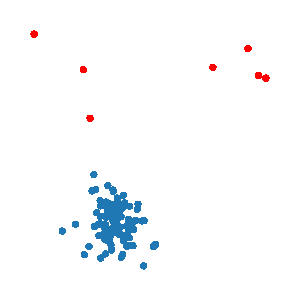
\includegraphics[width=\textwidth]{data/chapter_intro/point_anomalies.pdf}
         \caption{point anomalies}
         \label{fig:point_anomaly}
     \end{subfigure}
     \hfill
     \begin{subfigure}[b]{0.55\textwidth}
         \centering
         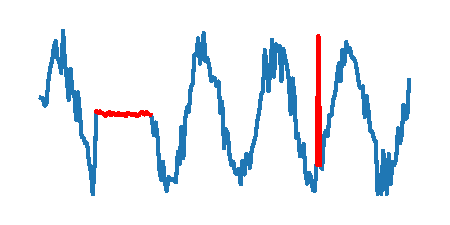
\includegraphics[width=\textwidth]{data/chapter_intro/group_anomalies.pdf}
         \caption{group (left) and contextual (right) anomaly}
         \label{fig:group_anomaly}
     \end{subfigure}

     \vspace{0.1in}

     \begin{subfigure}[b]{0.8\textwidth}
         \centering
         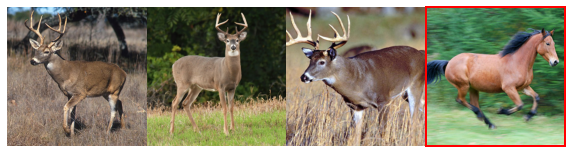
\includegraphics[width=\textwidth]{data/chapter_intro/semantic_anomalies.png}
         \caption{semantic anomaly}
         \label{fig:semantic_anomaly}
     \end{subfigure}

\caption{Examples of different types of anomalies.}
\label{fig:anomaly_examples}
\end{figure}

Different types of anomalies which require different approaches have been identified in literature~\cite{chandola2009anomaly,ruff2020unifying}. Examples are presented in Fig.~\ref{fig:anomaly_examples}.
\begin{itemize}
	\item \textbf{Point anomaly} is a single datapoint of $\mathcal{A}$, for example, an outlying measurement or a photograph of a cat among other images of dogs. This is the most often studied type of anomaly in the research literature. Note that a point anomaly can become an anomaly of the two following types if the datapoints in a dataset are somehow dependent (e.g. through time) or if some additional context about the data can be extracted.

	\item \textbf{Group anomalies} are a collection of correlated datapoints that are only anomalous together. Only a large number of malicious requests is enough to shut down a server in a DDoS atack~\cite{ahmed2018collective}. Other research~\cite{quellec2016multiple,wan2020weakly} focuses on finding anomalies under the multiple-instance learning (MIL)~\cite{carbonneau2018multiple} paradigm, where individual datapoints (called bags) are comprised of a variable number of observations or measurements (called instances). This calls for an aggregation method, on top of which an anomaly detector can operate.

	\item \textbf{Contextual} anomaly is a kind of anomaly that is only anomalous in a certain context. A person measuring over 195~cm is an outlier in almost any place except a locker room of a basketball team. If a target dataset consists of pictures of birds photographed mid-flight -- is a bird sitting on grass an anomaly? Or a different flying object, such as an airplane? The answers to those questions depend on what problem is actually being solved. Contextual anomalies often arise in time series~\cite{tsay2000outliers} or in spatial data~\cite{chawla2006slom}.

	\item \textbf{Semantic} anomalies arise in image data and are opposed to \textbf{sensory} anomalies. While sensory anomalies appear in low-level image features such as edges or textures (e.g. breaks or defects), semantic anomalies can be detected in the high-level information of an image (e.g. an object of a different category than what appears in the  training dataset). Semantic anomalies can be hard to detect, as they can be very similar to normal data~\cite{ahmed2020detecting}. We will cover their detection in chapters~\ref{sec:chapter_comparison} and~\ref{sec:chapter_sgvaegan}.
\end{itemize}


\section{Objectives}
In this short section, we summarize the objectives and goals of this work. The logical structure follows them, as each objective is covered by one or more chapters. The main objectives are the following:

\begin{enumerate}
	\item Providing a compilation of the current state-of-the art for both classical (shallow) models and (deep) generative models for anomaly detection. This is important in order to understand the theoretical properties of current methods. Also, by compiling all this information in one place, this work can then serve as an introduction to the topic of anomaly detection as well as to generative modelling. We also hope to provide some deeper insight into the behaviour of generative models in anomaly detection, as we believe that most of the current surveys are lacking in this respect.
	\item Conducting an extensive experimental comparison of selected methods under different operating conditions. This is meant to test the strengths and weaknesses of the individual methods in a broad range of conditions, such as varying data type, anomaly type and amount. The desired outcome of such an analysis is providing a direction in which deep generative models can bring added value, either in performance, explainability or other areas. 
	\item Finally, armed with the knowledge gained in the course of the work, the main goal is to propose a novel anomaly detector based on deep generative models. To validate that it solves the specific anomaly detection problem for which it is designed, an experimental comparison is needs to be conducted again. 
\end{enumerate}
